\chapter{Preliminaries}

\section{Introduction}
    This thesis is organized as follows.
    After necessary background material on Coxeter groups is presented in Section~\ref{sec:coxeter}, we introduce the class of fully commutative elements in Section~\ref{sec:FC}. Then, in Section~\ref{sec:heaps}, we discuss a visual representation for  elements of Coxeter groups, called heaps.
    The cyclically fully commutative elements, introduced in Section~\ref{sec:CFC}, are exactly those elements that are fully commutative when written in a circle and can be thought of as a generalization of Coxeter elements.
    In Section~\ref{sec:Sn}, we explore the connection between Coxeter groups of type $A_n$ and the symmetric group $S_{n+1}$. We also state a conjecture about the permutations corresponding of cyclically fully commutative elements (Conjecture~\ref{conjecture}).
    Finally, in Section~\ref{sec:chunks}, we introduce the notion of cylindrical heaps and ring equivalence in order to state the main result of this thesis (Theorem~\ref{thm:conjiffring}), which says that two cyclically fully commutative elements of a Coxeter group of type $A_n$ are conjugate if and only if their corresponding cylindrical heaps are ring equivalent.
    The last section states and proves several lemmas used to prove the main result.

\section{Coxeter groups}\label{sec:coxeter}
    A \emph{Coxeter system} is a pair $(W,S)$ consisting of a finite set $S$ of generating involutions and a group $W$, called a \emph{Coxeter group}, with presentation
    $$W = \gen{S \mid (st)^{m(s,t)} = e ~\text{for}~ m(s,t) < \infty },$$
    where $e$ is the identity, $m(s,t) = 1$ if and only if $s = t$, and $m(s,t) = m(t,s)$.
    It follows that the elements of $S$ are distinct as group elements and that $m(s,t)$ is the order of $st$~\cite{Humphreys1990}.
    We call $m(s,t)$ the \emph{bond strength} of $s$ and $t$.
    Coxeter groups are generalizations of reflection groups. Each generator $s \in S$ can be thought of as a reflection. Recall that the composition of two reflections is a rotation by twice the angle between the corresponding hyperplanes. So, if $s,t \in S$, we can think of $st$ as a rotation, where $m(s,t)$ is the order of the rotation.

    Since elements of $S$ have order two, the relation $(st)^{m(s,t)} = e$ can be written as
\begin{equation}\label{braid} \underbrace{sts \cdots}_{m(s,t)} = \underbrace{tst \cdots}_{m(s,t)} \end{equation}
    with $m(s,t) \geq 2$ factors.
    If $m(s,t) = 2$, then $st = ts$ is called a \emph{commutation relation} since $s$ and $t$ commute. If $m(s,t) \geq 3$, then the relation in \eqref{braid} is called a \emph{braid relation}.
    We will write $\gen{st}_{m(s,t)}$ to denote the word $sts \cdots$ consisting of $m(s,t)$ factors.
    Replacing $\gen{st}_{m(s,t)}$ with $\gen{ts}_{m(s,t)}$ will be referred to as a \emph{commutation} if $m(s,t) = 2$ and a \emph{braid move} if $m(s,t) \geq 3$.
    
    We can represent the Coxeter system $(W,S)$ with a unique \emph{Coxeter graph} $\Gamma$ having
\begin{enumerate}[leftmargin=0.75in,label=(\alph*)]
    \item vertex set $S = \{s_1, \ldots, s_n\}$ and
    \item edges $\{s_i,s_j\}$ for each $m(s_i,s_j) \geq 3$.
\end{enumerate} 
    Each edge $\{s_i,s_j\}$ is labeled with its corresponding bond strength $m(s_i,s_j)$. Since bond strength 3 is the most common, we typically omit the labels of 3 on those edges.
    
    There is a one-to-one correspondence between Coxeter systems and Coxeter graphs.
    Given a Coxeter graph $\Gamma$, we can construct the corresponding Coxeter system $(W,S)$.
    In this case, we say that $(W,S)$, or just $W$, is of type $\Gamma$. If $(W,S)$ is of type $\Gamma$, for emphasis, we may write $(W,S)$ as $(W(\Gamma),S(\Gamma))$.
    Note that generators $s_i$ and $s_j$ are connected by an edge in the Coxeter graph $\Gamma$ if and only if $s_i$ and $s_j$ do not commute~\cite{Humphreys1990}.
    Also, if $\Gamma$ is connected, then we say that $\Gamma$, or $W(\Gamma)$, is \emph{irreducible}.

    The Coxeter system of type $A_n$ is given by the Coxeter graph in Figure~\ref{fig:A}. We can construct $(W(A_n),S(A_n))$ having the generating set $S(A_n) = \{s_1, s_2, \ldots, s_n\}$ and defining relations
\begin{enumerate}[leftmargin=0.75in, label=(\alph*)]
    \item $s_is_i = e$ for all $i$;
    \item $s_is_j = s_js_i$ when $\abs{i-j} > 1$;
    \item $s_is_js_i = s_js_is_j$ when $\abs{i-j} = 1$.
\end{enumerate}
    The Coxeter group $W(A_n)$ is isomorphic to the symmetric group $S_{n+1}$ under the mapping that sends $s_i$ to the adjacent transposition $(i~i+1)$.
    This thesis focuses specifically on Coxeter systems of type $A_n$.

\begin{definition} Let $S^*$ denote the free monoid over $S$. If a word $\w=s_{x_1}s_{x_2}\cdots s_{x_m}\in S^*$ is equal to $w$ when considered as an element of $W$, we say that $\w$ is an \emph{expression} for $w$.
    (Expressions will be written in {\sf sans serif} font for clarity.) Furthermore, if $m$ is minimal among all possible expressions for $w$, we say that $\w$ is a \emph{reduced expression} for $w$, and we call $m$ the \emph{length} of $w$, denoted $\ell(w)$.
\end{definition}

    Each element $w \in W$ can have several different reduced expressions that represent it.
    The following theorem is called Matsumoto's Theorem.

\begin{theorem}[Matsumoto,~\cite{Boothby2012}] \label{thm:matsumoto} In a Coxeter group $W$, any two reduced expressions for the same group element differ by a sequence of commutations and braid moves. \qed
\end{theorem}

    It follows from Matsumoto's Theorem that all reduced expressions for $w \in W$ have the same number of generators appearing in the expression.
    Let $w \in W$ and let $\w$ be a reduced expression for $w$. Then the \emph{support} of $\w$, denoted $\supp(\w)$, is the set of generators that appear in $\w$.
    Also from Matsumoto's Theorem we have that $s$ appears in a reduced expression for $w$ if and only if $s$ appears in every reduced expression for $w$, so we can define the support of a group element.
    Define $\supp(w)$ to be the set of generators appearing in any reduced expression for $w$.
    If $\supp(w) = S$, we say that $w$ has \emph{full support}.
    
    Given a reduced expression $\w$ for $w \in W$, we define a \emph{subexpression} of $\w$ to be any subsequence of $\w$. We will refer to a subexpression consisting of a string of consecutive symbols from $\w$ as a \emph{subword} of $\w$.

\begin{example}\label{ex:subword} Let $w \in W(A_6)$ and let $\w = s_1 s_2 s_4 s_5 s_2 s_6 s_5$ be an expression for $w$. Then we have $$s_1 \textcolor{magenta}{s_2 s_4} s_5 s_2 s_6 s_5
    = s_1 s_4 \textcolor{magenta}{s_2 s_5} s_2 s_6 s_5
    = s_1 s_4 s_5 \textcolor{ggreen}{s_2 s_2} s_6 s_5
    = s_1 s_4 s_5 s_6 s_5,$$
    where the \textcolor{magenta}{pink} subword denotes applying a commutation to the corresponding generators to obtain the next expression and the \textcolor{ggreen}{green} subword denotes canceling two adjacent occurrences of the same generator.
    So, $\w$ is not reduced. It turns out that $s_1 s_4 s_5 s_6 s_5$ is a reduced expression for $w$ and $\supp(w) = \{s_1,s_2,s_4,s_5,s_6\}$. Hence $\ell(w) = 5$.
\end{example}

\begin{example} Let $W$ be the Coxeter group of type $A_4$, and let $w \in W$ have reduced expression $\w = s_1s_2s_3s_4s_2$. Then the set of all the reduced expressions for $w$ is
    $$\{s_1s_2s_3\textcolor{magenta}{s_4s_2}, s_1\textcolor{blue}{s_2s_3s_2}s_4, \textcolor{magenta}{s_1s_3}s_2s_3s_4, s_3s_1s_2s_3s_4\},$$
    where the \textcolor{magenta}{pink} subword denotes applying a commutation and the \textcolor{blue}{blue} subword denotes applying a braid relation to get to the next reduced expression. Then $\ell(w) = 5$ and $w$ has full support.
\end{example}
    
\begin{definition} A \emph{Coxeter element} is an element $w \in W$ for which every generator appears exactly once in each reduced expression for $w$. 
\end{definition}

    Note that $\supp(w) = S$ for a Coxeter element $w$. The set of Coxeter elements of $W$ is denoted by $\C(W)$.
    
\begin{example} \label{ex:Coxelt} Consider the Coxeter group of type $A_4$. Let $w_1, w_2, w_3, w_4 \in W(A_4)$ have reduced expressions $s_1s_2s_4s_3$, $s_2s_1s_3s_4$, $s_2s_4$, and $s_1s_2s_3s_4s_1s_2$, respectively.
    Then $w_1$ and $w_2$ are Coxeter elements because each has exactly one occurrence of each generator $s_1,s_2,s_3,s_4$ in its reduced expression.
    On the other hand, $w_3$ is not a Coxeter element because it does not have full support. Also, $w_4$ is not a Coxeter element because it has generators repeated; there are two occurrences each of $s_1$ and $s_2$ in its reduced expression.
\end{example}

\begin{example} Let $W$ be the Coxeter group of type $A_4$. Then the Coxeter elements of $W$ and their corresponding reduced expressions are shown in Figure~\ref{fig:coxeltsinA4}, where each column contains the reduced expressions for a single Coxeter element.
    There are $4! = 24$ reduced expressions for Coxeter elements in $W$, but there are only 8 Coxeter elements because some reduced expressions determine the same group element by commutation.
\begin{figure}[h!] \centering
$$\begin{array}{llllllll}
    s_1s_2s_3s_4 & s_4s_3s_2s_1 & s_1s_2s_4s_3 & s_2s_1s_3s_4 & s_3s_4s_2s_1 & s_4s_3s_1s_2 & s_1s_3s_2s_4 & s_2s_1s_4s_3 \\
         &      & s_1s_4s_2s_3 & s_2s_3s_1s_4 & s_3s_2s_4s_1 & s_4s_1s_3s_2 & s_3s_1s_2s_4 & s_2s_4s_1s_3 \\
         &      & s_4s_1s_2s_3 & s_2s_3s_4s_1 & s_3s_2s_1s_4 & s_1s_4s_3s_2 & s_1s_3s_4s_2 & s_2s_4s_3s_1 \\
         &      &      &      &      &      & s_3s_1s_4s_2 & s_4s_2s_1s_3 \\
         &      &      &      &      &      & s_3s_4s_1s_2 & s_4s_2s_3s_1
\end{array}$$
\caption{Coxeter elements and their reduced expressions in $W(A_4)$.} \label{fig:coxeltsinA4}
\end{figure}
\end{example}

\section{Fully commutative elements}\label{sec:FC}
    Let $(W,S)$ be a Coxeter system of type $\Gamma$ and let $w \in W$. Following~\cite{Stembridge1996}, we define a relation $\sim$ on the set of reduced expressions for $w$. Let $\w$ and $\w'$ be two reduced expressions for $w$. 
    We define $\w \sim \w'$ if we can obtain $\w'$ from $\w$ by applying a single commutation move of the form $s_is_j \mapsto s_js_i$, where $m(s_i,s_j) = 2$.
    Now, define the equivalence relation $\approx$ by taking the reflexive transitive closure of $\sim$. Each equivalence class under $\approx$ is called a \emph{commutation class}.
    Two reduced expressions are said to be \emph{commutation equivalent} if they are in the same commutation class.

\begin{example} \label{ex:comm_eq} Let $W$ be the Coxeter group of type $A_5$ and consider the reduced expressions $\w = s_1s_3s_2s_5s_4$ and $\w' = s_5s_1s_3s_4s_2$. Then $\w$ and $\w'$ are reduced expressions for the same element $w \in W$ and are commutation equivalent since
    $$s_1s_3\textcolor{magenta}{s_2s_5}s_4 = s_1s_3s_5\textcolor{magenta}{s_2s_4} = s_1\textcolor{magenta}{s_3s_5}s_4s_2 = \textcolor{magenta}{s_1s_5}s_3s_4s_2 = s_5s_1s_3s_4s_2,$$
    where the \textcolor{magenta}{pink} subwords denote applying a commutation to the corresponding generators to obtain the next expression.
\end{example}

\begin{example}\label{ex:nonFC} Let $W$ be the Coxeter group of type $A_4$ and let $w \in W$ have reduced expressions $\w = s_1 s_2 s_3 s_2 s_4$ and $\w' = s_1 s_3 s_2 s_3 s_4$.
    Then it is easily seen that $\w$ and $\w'$ are not commutation equivalent, so $w$ has more than one commutation class. Specifically, the commutation classes are $$\{s_1s_2s_3s_2s_4, s_1s_2s_3s_4s_2\} ~\text{and}~ \{s_1s_3s_2s_3s_4, s_3s_1s_2s_3s_4\}.$$
\end{example}

\begin{example}\label{ex:FC} Let $W$ be the Coxeter group of type $A_3$ and let $w \in W$ have reduced expression $\w = s_2s_1s_3s_2$. Then, by applying the commutation $s_1s_3 \mapsto s_3s_1$, $\w' = s_2s_3s_1s_2$ is also a reduced expression for $w$.
    There are no other reduced expressions for $w$ because we cannot apply any other commutations or braid moves. Therefore there is exactly one commutation class---namely, $\{s_2s_1s_3s_2, s_2s_3s_1s_2\}$.
\end{example}
    
    If $w$ has exactly one commutation class, then we say that $w$ is \emph{fully commutative}, or just FC.
    The set of all fully commutative elements of $W$ is denoted by $\FC(\Gamma)$, where $\Gamma$ is the corresponding Coxeter graph, or $\FC(W)$.
    For consistency, we say that a reduced expression $\w$ is FC if it is a reduced expression for some $w \in\FC(\Gamma)$.
    Note that the element in Example~\ref{ex:nonFC} is not FC since there are two commutation classes, while the element in Example~\ref{ex:FC} is FC since there is only one commutation class.

    Given some $w\in\FC(\Gamma)$ and a starting reduced expression for $w$, observe that the definition of fully commutative states that one only needs to perform commutations to obtain all the reduced expression for $w$, but the following theorem states that, when $w$ is FC, performing commutations is the only possible way to obtain another reduced expression for $w$.

\begin{theorem}[Stembridge,~\cite{Stembridge1996}] \label{thm:stem} An element $w \in W$ is FC if and only if no reduced expression for $w$ contains $\gen{s_i,s_j}_{m(s_i,s_j)}$ as a subword for all $s_i \neq s_j$ when $m(s_i,s_j) \geq 3$. \qed
\end{theorem}

    This theorem states that an element is FC if and only if there is no opportunity to apply a braid move.
    Notice that Coxeter elements are FC since there will never be opportunity to apply braid moves as, by definition, there is exactly one appearance of each generator.

\begin{example} \label{ex:FC2} Let $W$ be the Coxeter group of type $A_5$. Let $w \in W$ have reduced expression $\w = s_1 s_4 s_3 s_5 s_2 s_1 s_3 s_4$. Then we have 
    $$s_1 s_4 \textcolor{magenta}{s_3 s_5} s_2 s_1 s_3 s_4 = s_1 s_4 s_5 s_3 s_2 \textcolor{magenta}{s_1 s_3} s_4 = s_1 s_4 s_5 \textcolor{blue}{s_3 s_2 s_3} s_1 s_4,$$
    where the \textcolor{magenta}{pink} subword denotes applying a commutation to the corresponding generators to obtain the next expression.
    So, $w$ is not FC because there is opportunity to apply a braid move, highlighted in \textcolor{blue}{blue}.
\end{example}

    Stembridge classified the irreducible Coxeter groups that contain only finitely many fully commutative elements, called the \emph{FC-finite Coxeter groups}.
    This thesis is mainly concerned with $W(A_n)$, which is a finite group, so it has finitely many FC elements. However, there exist infinite Coxeter groups that contain only finitely many FC elements. 
    For example, Coxeter groups of type $E_n$ with $n \geq 9$ as shown in Figure~\ref{fig:E} are infinite, but they have only finitely many FC elements.

\begin{theorem}[Stembridge,~\cite{Stembridge1996}] \label{thm:FCfinite} The FC-finite irreducible Coxeter groups are of type $A_n$ with $n \geq 1$, $B_n$ with $n \geq 2$, $D_n$ with $n \geq 4$, $E_n$ with $n \geq 6$, $F_n$ with $n \geq 4$, $H_n$ with $n \geq 3$, and $I_2(m)$ with $5 \leq m < \infty$. The corresponding Coxeter graphs are shown in Figure~\ref{fig:coxgraphs}. \qed
\end{theorem}

\begin{figure}[h!]
\begin{tabular}{m{7cm} m{7cm}}
\begin{subfigure}{0.5\textwidth} \centering
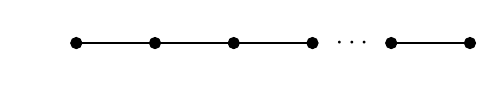
\begin{tikzpicture}[scale=1.0]%A_{n}
\draw[fill=black] \foreach \x in {1,2,...,6} {(\x,10) circle (2pt)};
\draw {(.5,10) node{}
(4.5,10) node{$\cdots$}
[-] (1,10) -- (4,10)
[-] (5,10) -- (6,10)
(1,10) node{}}; 
\end{tikzpicture}
\caption{$A_{n}$} \label{fig:A}
\end{subfigure} &

\begin{subfigure}{0.5\textwidth} \centering
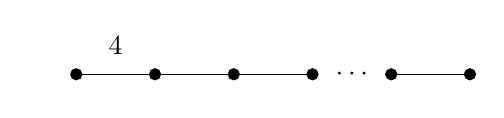
\begin{tikzpicture}[scale=1.0]%B_{n}
\draw [fill=black] \foreach \x in {1,2,...,6} {(\x,8.5) circle (2pt)};
\draw {(.5,8.5) node{}
(1.5,8.5) node[label=above:$4$]{}
(4.5,8.5) node{$\cdots$}
[-] (1,8.5) -- (4,8.5)
[-] (5,8.5) -- (6,8.5)
(2,8.5) node{}}; 
\end{tikzpicture}
\caption{$B_{n}$} \label{fig:B}
\end{subfigure} \\

    & \\ 

\begin{subfigure}{0.5\textwidth} \centering
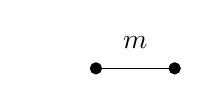
\begin{tikzpicture}[scale=1.0]
\draw[fill=black] \foreach \x in {1,2} {(\x,0) circle (2pt)};
\draw {(.25,0) node{}
(1.5,0) node[label=above:$m$]{}
[-] (1,0) -- (2,0)
(2,0) node{}};
\end{tikzpicture}
\caption{$I_{2}(m)$} \label{fig:I}
\end{subfigure} &

\begin{subfigure}{0.5\textwidth} \centering
\begin{tikzpicture}[scale=1.0]
\draw[fill=black] \foreach \x in {1,2,...,6} {(\x,6.5) circle (2pt)};%D_{n}
\draw[fill=black] (2,7.5) circle (2pt);
\draw {(.5,6.5) node{}
(4.5,6.5) node{$\cdots$}
[-] (1,6.5) -- (4,6.5)
[-] (5,6.5) -- (6,6.5)
[-] (2,6.5) -- (2,7.5)
(2,6.5) node{}};
\end{tikzpicture}
\caption{$D_{n}$} \label{fig:D}
\end{subfigure} \\

    & \\ 
    
\begin{subfigure}{0.5\textwidth} \centering
\begin{tikzpicture}[scale=1.0]%E_{n}
\draw[fill=black] \foreach \x in {1,2,...,6} {(\x,4.5) circle (2pt)};
\draw[fill=black] (3,5.5) circle (2pt);
\draw {(.5,4.5) node{}
(4.5,4.5) node{$\cdots$}
[-] (1,4.5) -- (4,4.5)
[-] (5,4.5) -- (6,4.5)
[-] (3,4.5) -- (3,5.5)
(3,4.5) node{}};
\end{tikzpicture}
\caption{$E_{n}$} \label{fig:E}
\end{subfigure} &

\begin{subfigure}{0.5\textwidth} \centering
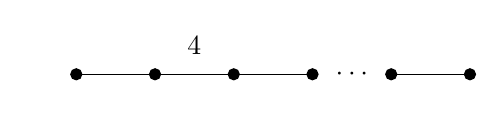
\begin{tikzpicture}[scale=1.0]%F_{n}
\draw[fill=black] \foreach \x in {1,2,...,6} {(\x,3) circle (2pt)};
\draw {(.5,3) node{}
(2.5,3) node[label=above:$4$]{}
(4.5,3) node{$\cdots$}
[-] (1,3) -- (4,3)
[-] (5,3) -- (6,3)
(3,3) node{}};
\end{tikzpicture}
\caption{$F_{n}$} \label{fig:F}
\end{subfigure} \\

    & \\ 

\begin{subfigure}{0.5\textwidth} \centering
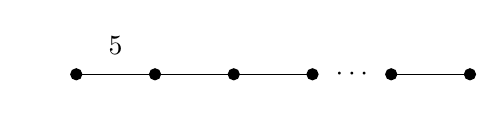
\begin{tikzpicture}[scale=1.0]
\draw[fill=black] \foreach \x in {1,2,...,6} {(\x,1.5) circle (2pt)};%H_{n}
\draw {(.5,1.5) node{}
(1.5,1.5) node[label=above:$5$]{}
(4.5,1.5) node{$\cdots$}
[-] (1,1.5) -- (4,1.5)
[-] (5,1.5) -- (6,1.5)
(2,1.5) node{}}; 
\end{tikzpicture}
\caption{$H_{n}$} \label{fig:H}
\end{subfigure}
\end{tabular}
\caption{Coxeter graphs corresponding to the irreducible FC-finite Coxeter groups.}
\label{fig:coxgraphs}
\end{figure}

    It is well known that the number of FC elements in $W(A_{n-1})$ is given by the Catalan number $C_n = \frac{1}{n+1} \binom{2n}{n}$.
    
    
\section{Heaps}\label{sec:heaps}
    We can now discuss another representation of elements of Coxeter groups. Each reduced expression is associated with a labeled partially ordered set called a heap. 
    We follow the development in~\cite{Ernst2010} and~\cite{Stembridge1996}.

\begin{definition} \label{def:heap} Let $(W,S)$ be a Coxeter system. Suppose $\w = s_{x_1} s_{x_2} \cdots s_{x_k}$ is a reduced expression for $w \in W$, and as in~\cite{Stembridge1996}, define a partial ordering $\prec$ on the indices $\{1,\ldots,k\}$ by the transitive closure of the relation $j \prec i$ if $i < j$ and $s_{x_i}$ and $s_{x_j}$ do not commute.
    In particular, $j \prec i$ if $i < j$ and $s_{x_i} = s_{x_j}$ by transitivity and the fact that $\w$ is reduced.
    This partial order with $i$ labeled $s_{x_i}$ is called the \emph{heap} of $\w$.
\end{definition}

    Note that for simplicity, we are omitting the labels of the underlying poset but retaining the labels of the corresponding generators.

\begin{example}\label{ex:firstheap} Let $\w = s_2 s_1 s_3 s_2 s_4 s_5$ be a reduced expression for $w \in W(A_5)$.  We see that $\w$ is indexed by $\{1, 2, 3, 4, 5, 6\}$ because $\ell(w)=6$. We see that $4 \prec 3$ since $3 < 4$ and $s_4$ and $s_3$ do not commute.
    The labeled Hasse diagram for the heap poset of $\w$ is shown in Figure~\ref{fig:hasse}.
\begin{center} \begin{figure}[h!] \centering
\begin{tikzpicture}
\draw (0,2)--(-1,1); \draw (0,2)--(1,1); \draw (-1,1)--(0,0); \draw (0,0)--(1,1); \draw (1,1)--(2,0); \draw (2,0)--(3,-1);
\draw [fill=black] (0,2) circle (1.5pt); \draw[color=black] (0,2.4) node {$s_2$};
\draw [fill=black] (-1,1) circle (1.5pt); \draw[color=black] (-1.4,1.2) node {$s_1$};
\draw [fill=black] (1,1) circle (1.5pt); \draw[color=black] (1.3,1.2) node {$s_3$};
\draw [fill=black] (0,0) circle (1.5pt); \draw[color=black] (0,0.5) node {$s_2$};
\draw [fill=black] (2,0) circle (1.5pt); \draw[color=black] (2.4,0.1) node {$s_4$};
\draw [fill=black] (3,-1) circle (1.5pt); \draw[color=black] (3.4,-0.8) node {$s_5$};
\end{tikzpicture}
\caption{The labeled Hasse diagram for the heap poset of $w = s_2 s_1 s_3 s_2 s_4 s_5$.} \label{fig:hasse}
\end{figure} \end{center}
\end{example}

    Let $\w$ be a fixed reduced expression for $w \in W(A_n)$. As in~\cite{Billey2007} and~\cite{Ernst2010}, we represent a heap for $\w$ as a set of lattice points embedded in $\{1,\ldots,n\} \times \N$.
    To do so, we assign (not necessarily unique) coordinates $(x,y) \in \{1,\ldots,n\} \times \N$ to each entry of the labeled Hasse diagram for the heap of $\w$ in such a way that
\begin{enumerate}[leftmargin=0.75in, label=(\alph*)]
    \item An entry with coordinates $(x,y)$ is labeled $s_i$ (or $i$) in the heap if and only if $x = i$; 
    \item An entry with coordinates $(x,y)$ is greater than an entry with coordinates $(x',y')$ in the heap if and only if $y > y'$.
\end{enumerate}
    It follows from the definition that there is an edge in the Hasse diagram from $(x,y)$ to $(x',y')$ if and only if $x = x' \pm 1$, $y > y'$, and there are no entries $(x'', y'')$ such that $x'' \in \{x, x'\}$ and $y'< y'' < y$.
    This implies that we can completely reconstruct the edges of the Hasse diagram and the corresponding heap poset from a lattice point representation.
    The lattice point representation of a heap allows us to visualize potentially cumbersome arguments. Note that our heaps are upside-down versions of the heaps that appear in~\cite{Billey2007} and several other papers. That is, in this thesis entries on top of a heap correspond to generators occurring to the left, as opposed to the right, in the corresponding reduced expression.
    One can form similar lattice point representations for heaps when $\Gamma$ is a straight line Coxeter graph.
    
    Let $\w = s_{x_1} \cdots s_{x_n}$ be any reduced expression for $w \in W(A_{n})$. We let $H(\w)$ denote a lattice representation of the heap poset in $\{1,\ldots,n\} \times \N$ described in the paragraph above.
    There are many possible coordinate assignments for the entries of $H(\w)$, yet the $x$-coordinates for each entry will be fixed. If $s_{x_i}$ and $s_{x_j}$ are adjacent generators in the Coxeter graph with $i<j$, then we must place the point labeled by $s_{x_i}$ at a level that is \emph{above} the level of the point labeled by $s_{x_j}$.
    In particular, two entries labeled by the same generator may only differ by the amount of vertical space between them while maintaining their relative vertical position to adjacent entries in the heap.
    
    Because generators that are not adjacent in the Coxeter graph commute, points whose $x$-coordinates differ by more than one can slide past each other or land at the same level.
    To visualize the labeled heap poset of a lattice representation we will enclose each entry of the heap in a block in such a way that if one entry covers another, the blocks overlap halfway.

\begin{remark} It follows from Proposition 2.2 in~\cite{Stembridge1996} that heaps are well-defined up to commutation class.
    That is, if $\w$ and $\w'$ are two reduced expressions for $w \in W$ that are in the same commutation class, then the labeled heaps of $\w$ and $\w'$ are equal.
    In particular, if $w$ is FC, then it has a single commutativity class, and so there is a unique heap associated to $w$.
    In this case, if $w$ is FC, then we may write $H(w)$ to denote the heap of any reduced expression for $w$.
\end{remark}

    There are potentially many different ways to represent a heap, each differing by the vertical placement of blocks. For example, we can place blocks in vertical positions that are as high as possible, as low as possible, or some combination of high/low. In this thesis, we choose what we view to be the best representation of the heap for each example.

\begin{example}\label{ex:heap} Let $W$ be the Coxeter group of type $A_5$ and $\w = s_1s_2s_3s_1s_2s_4s_5$ be a reduced expression for $w \in \FC(W)$.
    We will construct one possible lattice point representation for $H(w)$.
    Starting from the right hand side, the first generator is $s_5$, so we place a block, labeled with a 5, in position $(5,1)$. Observe that the $x$-coordinate is forced to be 5 since the block corresponds to the generator $s_5$, but we have a choice for the $y$-coordinate. We choose to place it as low as possible to get
\begin{center} \begin{tabular}{m{2.75cm} m{0.5cm}} \begin{tikzpicture}
    \node at (0.5,-1.5) {$s_1$}; \node at (1,-1.5) {$s_2$}; \node at (1.5,-1.5) {$s_3$}; \node at (2,-1.5) {$s_4$}; \node at (2.5,-1.5) {$s_5$};
    \draw[dotted, line width=0.5pt] (0.5,-1.2) -- (0.5,2);
    \draw[dotted, line width=0.5pt] (1,-1.2)   -- (1,2);
    \draw[dotted, line width=0.5pt] (1.5,-1.2) -- (1.5,2);
    \draw[dotted, line width=0.5pt] (2,-1.2)   -- (2,2);
    \draw[dotted, line width=0.5pt] (2.5,-1.2) -- (2.5,2);
    \sq{2}{0}; \node at (2.5,-0.5) {$5$};
\end{tikzpicture} & . 
\end{tabular} \end{center}

    \noindent Now, moving right to left, the next generator is $s_4$, so, similarly, we place a block, labeled with a 4, in position $(4,2)$. The $x$-coordinate must be 4, and we must place it at $y \geq 2$ because $s_4$ and $s_5$ do not commute, and so the $s_4$ block will be on a level above $s_5$, overlapping it halfway. We choose to place it as low as possible to get
\begin{center} \begin{tabular}{m{2.75cm} m{0.5cm}} \begin{tikzpicture}
    \node at (0.5,-1.5) {$s_1$}; \node at (1,-1.5) {$s_2$}; \node at (1.5,-1.5) {$s_3$}; \node at (2,-1.5) {$s_4$}; \node at (2.5,-1.5) {$s_5$};
    \draw[dotted, line width=0.5pt] (0.5,-1.2) -- (0.5,2);
    \draw[dotted, line width=0.5pt] (1,-1.2)   -- (1,2);
    \draw[dotted, line width=0.5pt] (1.5,-1.2) -- (1.5,2);
    \draw[dotted, line width=0.5pt] (2,-1.2)   -- (2,2);
    \draw[dotted, line width=0.5pt] (2.5,-1.2) -- (2.5,2);
    \sq{2}{0};   \node at (2.5,-0.5) {$5$};
    \sq{1.5}{1}; \node at (2,0.5)    {$4$};
\end{tikzpicture} & . 
\end{tabular} \end{center}

    \noindent The next two generators, moving to the left, are $s_2$ and $s_1$.  Since $s_2$ and $s_4$ commute, we place the corresponding blocks on the same level as each other (or with the same $y$-coordinate). We could have placed the $s_2$ block lower in the heap since there is nothing blocking it, but we choose to place it on the same level as the $s_4$ block because they commute.
    Since the $s_4$ block has 2 as its $y$-coordinate, we place the $s_2$ block in position $(2,2)$.
    Since $s_2$ and $s_1$ do not commute, we must place the $s_1$ block above the $s_2$ block. We choose to place the $s_1$ block in position $(1,3)$.
    We get
\begin{center} \begin{tabular}{m{2.9cm} m{0.5cm}} 
\begin{tikzpicture}
    \node at (0.5,-1.5) {$s_1$}; \node at (1,-1.5) {$s_2$}; \node at (1.5,-1.5) {$s_3$}; \node at (2,-1.5) {$s_4$}; \node at (2.5,-1.5) {$s_5$};
    \draw[dotted, line width=0.5pt] (0.5,-1.2) -- (0.5,2.5);
    \draw[dotted, line width=0.5pt] (1,-1.2)   -- (1,2.5);
    \draw[dotted, line width=0.5pt] (1.5,-1.2) -- (1.5,2.5);
    \draw[dotted, line width=0.5pt] (2,-1.2)   -- (2,2.5);
    \draw[dotted, line width=0.5pt] (2.5,-1.2) -- (2.5,2.5);
    \sq{2}{0};   \node at (2.5,-0.5) {$5$};
    \sq{1.5}{1}; \node at (2,0.5)    {$4$};
    \sq{0.5}{1};   \node at(1,0.5)   {$2$};
    \sq{0}{2};   \node at(0.5,1.5)   {$1$};
\end{tikzpicture} & .
\end{tabular} \end{center}

    \noindent Continuing to place blocks in the same manner, a heap representation that corresponds to $\w$ is
\begin{center} \begin{tabular}{m{2.9cm} m{0.5cm}}  \begin{tikzpicture}
    \node at (0.5,-1.5) {$s_1$}; \node at (1,-1.5) {$s_2$}; \node at (1.5,-1.5) {$s_3$}; \node at (2,-1.5) {$s_4$}; \node at (2.5,-1.5) {$s_5$};
    \draw[dotted, line width=0.5pt] (0.5,-1.2) -- (0.5,4.2);
    \draw[dotted, line width=0.5pt] (1,-1.2)   -- (1,4.2);
    \draw[dotted, line width=0.5pt] (1.5,-1.2) -- (1.5,4.2);
    \draw[dotted, line width=0.5pt] (2,-1.2)   -- (2,4.2);
    \draw[dotted, line width=0.5pt] (2.5,-1.2) -- (2.5,4.2);
    \sq{2}{0};   \node at (2.5,-0.5) {$5$};
    \sq{1.5}{1}; \node at (2,0.5)    {$4$};
    \sq{0.5}{1}; \node at (1,0.5)    {$2$};
    \sq{0}{2};   \node at (0.5,1.5)  {$1$};
    \sq{1}{2};   \node at (1.5,1.5)  {$3$};
    \sq{0.5}{3}; \node at (1,2.5)    {$2$};
    \sq{0}{4};   \node at (0.5,3.5)  {$1$};
\end{tikzpicture} & .
\end{tabular} \end{center}
\end{example}
    
    Conversely, given a heap, we can write an expression for the group element.
    By starting on the top and moving left to right and down, we write the corresponding generators. We get an expression that is commutation equivalent to any expression to which the heap corresponds.
    
\begin{example} Given the heap in Figure~\ref{fig:heapToRedExp}, we obtain the reduced expression $s_2 s_3 s_5 s_4$, which is commutation equivalent to $s_2s_5s_3s_4$ and $s_5s_2s_3s_4$, all of which yield the same heap. In fact, all reduced expressions yield the same heap since this particular element is FC.

\begin{center} \begin{figure}[H] \centering
\begin{tikzpicture}
    \sq{2}{2};   \node at (2.5,1.5)  {$5$};
    \sq{1.5}{1}; \node at (2,0.5)    {$4$};
    \sq{0.5}{3}; \node at (1,2.5)    {$2$};
    \sq{1}{2};   \node at (1.5,1.5)  {$3$};
\end{tikzpicture}
\caption{The heap for an FC element.}\label{fig:heapToRedExp}
\end{figure} \end{center}
\end{example}
   
\begin{example} We return to Example~\ref{ex:heap}. Note that $\w = s_1s_2s_3s_1s_2s_4s_5$ is not fully commutative because there is opportunity to apply a braid relation.
    We have
    \begin{equation} \label{eq:nonuniqueheapex} 
        s_1s_2\textcolor{magenta}{s_3s_1}s_2s_4s_5 = \textcolor{blue}{s_1s_2s_1}
        s_3s_2s_4s_5 = s_2s_1s_2s_3s_2s_4s_5,
    \end{equation}
where the \textcolor{magenta}{pink} subword denotes applying a commutation to obtain the next expression and the \textcolor{blue}{blue} subword denotes applying a braid relation to obtain the next expression.
    Since $w$ is not FC, we can represent $w$ with a different heap using the last reduced expression $s_2s_1s_2s_3s_2s_4s_5$ in (\ref{eq:nonuniqueheapex}).
    We get the heap shown in Figure~\ref{fig:nonuniqueheapex} as another representation of $w$. Note that we can see the braid relation $s_2s_1s_2 = s_1s_2s_1$ in the heap, highlighted in \textcolor{blue}{blue}, that we applied in (\ref{eq:nonuniqueheapex}).
\begin{center} \begin{figure}[H] \centering
\begin{tikzpicture}
    \sq{2}{0};     \node at (2.5,-0.5) {$5$};
    \sq{1.5}{1};   \node at (2,0.5)    {$4$};
    \sq{0.5}{1};   \node at (1,0.5)    {$2$};
    \sqbl{0}{4};   \node at (0.5,3.5)  {$1$};
    \sq{1}{2};     \node at (1.5,1.5)  {$3$};
    \sqbl{0.5}{3}; \node at (1,2.5)    {$2$};
    \sqbl{0.5}{5}; \node at (1,4.5)    {$2$};
\end{tikzpicture}
\caption{A second heap for the element in Example~\ref{ex:heap}.} \label{fig:nonuniqueheapex}
\end{figure} \end{center}
\end{example}

\begin{definition}\label{def:subheap} Let $\w = s_{x_{1}} \cdots s_{x_{n}}$ be a reduced expression for $w \in W$.  We define a heap $H'$ to be a \emph{subheap} of $H(\w)$ if $H' = H(\w')$, where $\w' = s_{y_1}s_{y_2} \cdots s_{y_k}$ is a subexpression of $\w$. We emphasize that the subexpression need not be a subword.
\end{definition} 

    We say that a subposet $Q$ of a poset $P$ is \emph{convex} if $y \in Q$ whenever $x < y < z$ in $P$ and $x, z \in Q$. We will refer to a subheap as a \emph{convex subheap} if the underlying subposet is convex.  

\begin{example} Let $w \in W(A_6)$ have reduced expression $\w = s_2 s_3 \textcolor{blue}{s_5 s_4} s_6 \textcolor{blue}{s_5}$. Since there is no opportunity to apply a braid relation in any reduced expression for $w$, $w$ is FC, and so there is a unique heap.
    The heap $H(w)$ is shown in Figure~\ref{fig:FCheapex}. Notice that we chose to place all the blocks in this heap as low as possible.

\begin{center} \begin{figure}[H] \centering
\begin{tikzpicture}
    \sq{0.5}{0}; \node at (1,-0.5)  {\footnotesize $5$};
    \sq{1}{1};   \node at (1.5,0.5) {\footnotesize $6$};
    \sq{0}{1};   \node at (0.5,0.5) {\footnotesize $4$};
    \sq{0.5}{2}; \node at (1,1.5)   {\footnotesize $5$};
    \sq{-0.5}{2};\node at (0,1.5)   {\footnotesize $3$};
    \sq{-1}{3};  \node at (-0.5,2.5){\footnotesize $2$};
\end{tikzpicture}
\caption{The heap of an FC element of $W(A_6)$.}\label{fig:FCheapex}
\end{figure} \end{center}
   
    Now, let $\w' = s_5 s_4 s_5$ be the subexpression of $\w$ that results from picking the third, fourth, and last generators of $\w$, highlighted in \textcolor{blue}{blue}. Then $H(\w')$ is shown in Figure~\ref{fig:nonconvexsubheapex} and is a subheap of $H(w)$, but $H(\w')$ is not convex since there is a block in $H(w)$ corresponding to the generator $s_6$ that occurs between the two occurrences of $s_5$ but does not have a block representing it in $H(\w')$.
    However, if we include the generator $s_6$, we get $\w'' = s_5 s_4 s_6 s_5$, and $H(\w'')$ is a convex subheap of $H(w)$, as shown in Figure~\ref{fig:convexsubheapex}.

\begin{center} \begin{figure}[H] \centering
\begin{subfigure}{0.4\textwidth} \centering
\begin{tikzpicture}
    \sq{0.5}{2}; \node at (1,1.5)   {\footnotesize $5$};
    \sq{0}{1};   \node at (0.5,0.5) {\footnotesize $4$};
    \sq{0.5}{0}; \node at (1,-0.5)  {\footnotesize $5$};
\end{tikzpicture}
\caption{}\label{fig:nonconvexsubheapex}
\end{subfigure}
\begin{subfigure}{0.4\textwidth} \centering
\begin{tikzpicture}
    \sq{0.5}{2}; \node at (1,1.5)   {\footnotesize $5$};
    \sq{0}{1};   \node at (0.5,0.5) {\footnotesize $4$};
    \sq{0.5}{0}; \node at (1,-0.5)  {\footnotesize $5$};
    \sq{1}{1};   \node at (1.5,0.5) {\footnotesize $6$};
\end{tikzpicture}
\caption{}\label{fig:convexsubheapex}
\end{subfigure}
\caption{Non-convex and convex subheaps of the heap in Figure~\ref{fig:FCheapex}.}
\end{figure}
\end{center}
    
    Notice that if we remove the block labeled by 6 from the original heap, then the heap in Figure~\ref{fig:nonconvexsubheapex} is a convex subheap of $H(w)$.
\end{example}

    From this point on, if there will be no confusion, we will not specify the exact subexpression from which a subheap arises.
    The following proposition follows from the proof of Proposition 3.3 in~\cite{Stembridge1996}.

\begin{proposition}\label{prop:convexsubheapiff} Let $w \in \FC(W)$.  Then $H'$ is a convex subheap of $H(w)$ if and only if $H'$ is the heap for some subword of some reduced expression for $w$. \qed
\end{proposition}

    The following proposition follows from Lemma 2.4.5 in~\cite{Ernst2010}. It will help us identify when a heap corresponds to a fully commutative element in $W(A_n)$.

\begin{proposition} \label{prop:convexsubheap} Let $w \in \FC(A_n)$. Then $H(w)$ cannot contain either of the convex subheaps shown in Figure~\ref{fig:convexnotinFCheaps}, where $1 \leq i \leq n-1$ and \begin{tabular}{m{0.5cm}} \begin{tikzpicture}[scale=0.6] \bsq{0}{0}; \end{tikzpicture} \end{tabular} is used to emphasize the absence of a block in the corresponding position in $H(w)$. \qed
\end{proposition}
\begin{center} \begin{figure}[H] \centering
\begin{subfigure}{0.3\textwidth} \centering
\begin{tikzpicture}
    \sq{0.5}{2}; \node at (1,1.5) {\footnotesize $i+1$};
    \sq{0}{1}; \node at (0.5,0.5) {\footnotesize $i$};
    \sq{0.5}{0}; \node at (1,-0.5) {\footnotesize $i+1$};
    \bsq{1}{1};
\end{tikzpicture}\caption{}
\end{subfigure}
\begin{subfigure}{0.3\textwidth} \centering
\begin{tikzpicture}
    \sq{0}{2}; \node at (0.5,1.5) {\footnotesize $i$};
    \sq{0.5}{1}; \node at (1,0.5) {\footnotesize $i+1$};
    \sq{0}{0}; \node at (0.5,-0.5) {\footnotesize $i$};
    \bsq{-0.5}{1};
\end{tikzpicture}\caption{}
\end{subfigure}
\caption{The convex subheaps not contained in heaps of FC elements.}\label{fig:convexnotinFCheaps}
\end{figure} \end{center}

    The following lemma will become useful in proofs in later sections.

\begin{lemma}\label{lem:stst}
If $m(s_i,s_j) = 3$, then $s_is_js_is_j = s_js_i$.
\end{lemma}

\begin{proof} Consider the expression $s_is_js_is_j$. Applying a braid relation to the first three generators and simplifying, we get $s_is_js_is_j = s_js_is_js_j = s_js_i$.
\end{proof}

    Recall that we defined heaps for reduced expressions. However, it will be useful for us to extend the stacked blocks representation of a heap to non-reduced expressions, which we do in the obvious way. If $\w$ and $\w'$ are two expressions, not necessarily reduced, for $w \in W$, then we will write $H(\w) \equiv H(\w')$.

    Using this idea, we can write Lemma~\ref{lem:stst} in terms of heaps. If $m(s_i,s_j) = 3$, then we have the equivalent heaps shown in Figure~\ref{fig:lemststheaps}.
\begin{center} \begin{figure}[H] \centering
\begin{subfigure}{0.4\textwidth} \centering
\begin{tabular}{m{2cm}m{0.5cm}m{1cm}}
\begin{tikzpicture}
    \sq{0}{2};    \node at (0.5,1.5) {$i$};
    \sq{0.5}{1};  \node at (1,0.5)   {$j$};
    \sq{0}{0};    \node at (0.5,-0.5){$i$};
    \sq{0.5}{-1}; \node at (1,-1.5)  {$j$};
    \bsq{1}{0};
\end{tikzpicture} & $\equiv$ &
\begin{tikzpicture}
    \sq{0.5}{1};  \node at (1,0.5)    {$j$};
    \sq{0}{0};    \node at (0.5,-0.5) {$i$};
\end{tikzpicture}
\end{tabular} \caption{}
\end{subfigure}
\begin{subfigure}{0.4\textwidth} \centering
\begin{tabular}{m{2cm}m{0.5cm}m{1cm}}
\begin{tikzpicture}
    \sq{0.5}{2};  \node at (1,1.5)   {$j$};
    \sq{0}{1};    \node at (0.5,0.5) {$i$};
    \sq{0.5}{0};  \node at (1,-0.5)  {$j$};
    \sq{0}{-1};   \node at (0.5,-1.5){$i$};
    \bsq{-0.5}{0};
\end{tikzpicture} & $\equiv$ &
\begin{tikzpicture}
    \sq{0}{1};    \node at (0.5,0.5) {$i$};
    \sq{0.5}{0};  \node at (1,-0.5)  {$j$};
\end{tikzpicture}
\end{tabular} \caption{}
\end{subfigure}
\caption{Lemma~\ref{lem:stst} in terms of heaps.}\label{fig:lemststheaps}
\end{figure} \end{center}

    Let $w \in W(A_n)$ with expression $\w$. If $s_is_js_is_j$ is a subword of $\w$ with $m(s_i,s_j) = 3$, then we refer to $s_is_js_is_j$ as an \emph{extra long $s_is_j$-chain}.

\begin{remark} From now on, for brevity, we may write $i$ in place of the generator $s_i$. For example, we may write $123$ in place of $s_1s_2s_3$.
\end{remark}